\documentclass[12pt, a4paper, oneside]{ctexart}
\usepackage{amsmath, amsthm, amssymb, bm, color, framed, graphicx, hyperref, mathrsfs, float}
\pagestyle{plain}

% multi-column
\usepackage{tasks}
% itemize
\NewTasksEnvironment[label=(\arabic*), label-width=3ex]{exercise}

\everymath{\displaystyle}

\title{\textbf{第三次随堂测试}}
\author{U08M11002 Fall 2023}
\linespread{1}
\definecolor{shadecolor}{RGB}{241, 241, 255}

\newcounter{problemname}
\newenvironment{problem}{\stepcounter{problemname}\par\noindent\textbf{题目\arabic{problemname}. }}{\\\par}
\newenvironment{warning}{\begin{shaded}\par\noindent\textbf{提交作业方式:}}{\end{shaded}\par}

\begin{document}

\maketitle

\hspace{1em}

\begin{problem}
求下列两图中所示周期信号的傅里叶级数:
    \begin{figure}[H]
        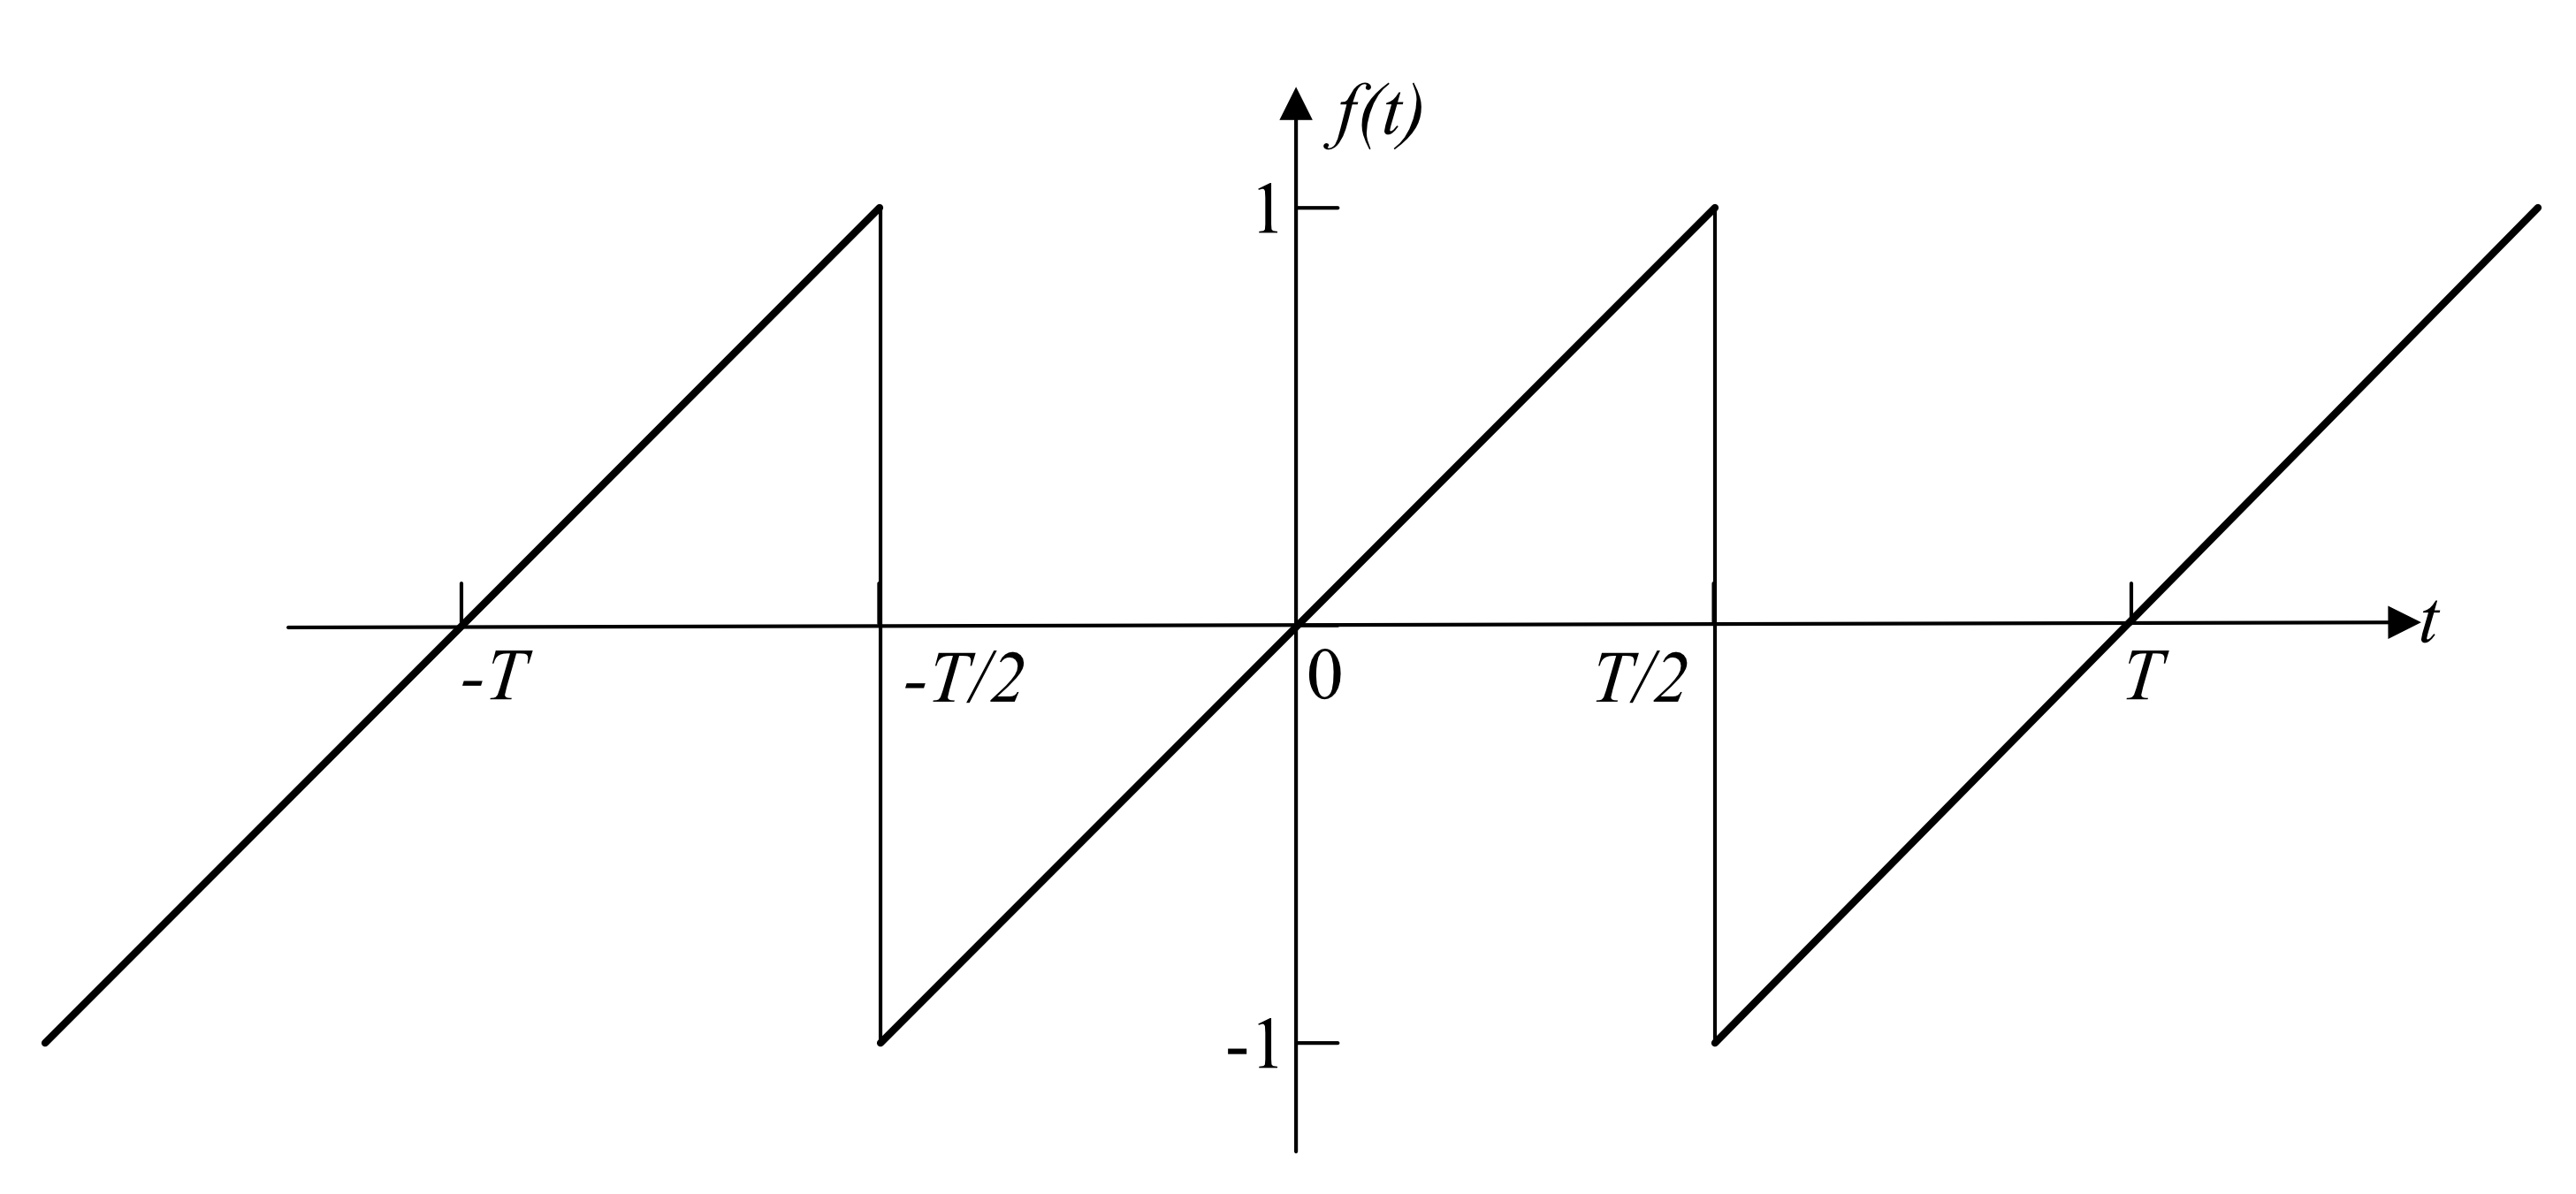
\includegraphics[width=10cm]{assets/hw4img1.png}
        \centering
    \end{figure}
\quad
\end{problem}

\begin{problem}
已知单位冲激序列$\delta_T(t) = \sum_{k=-\infty}^{\infty}\delta(t-KT)$如下图所示.求其傅里叶级数与频谱。
	\begin{figure}[H]
		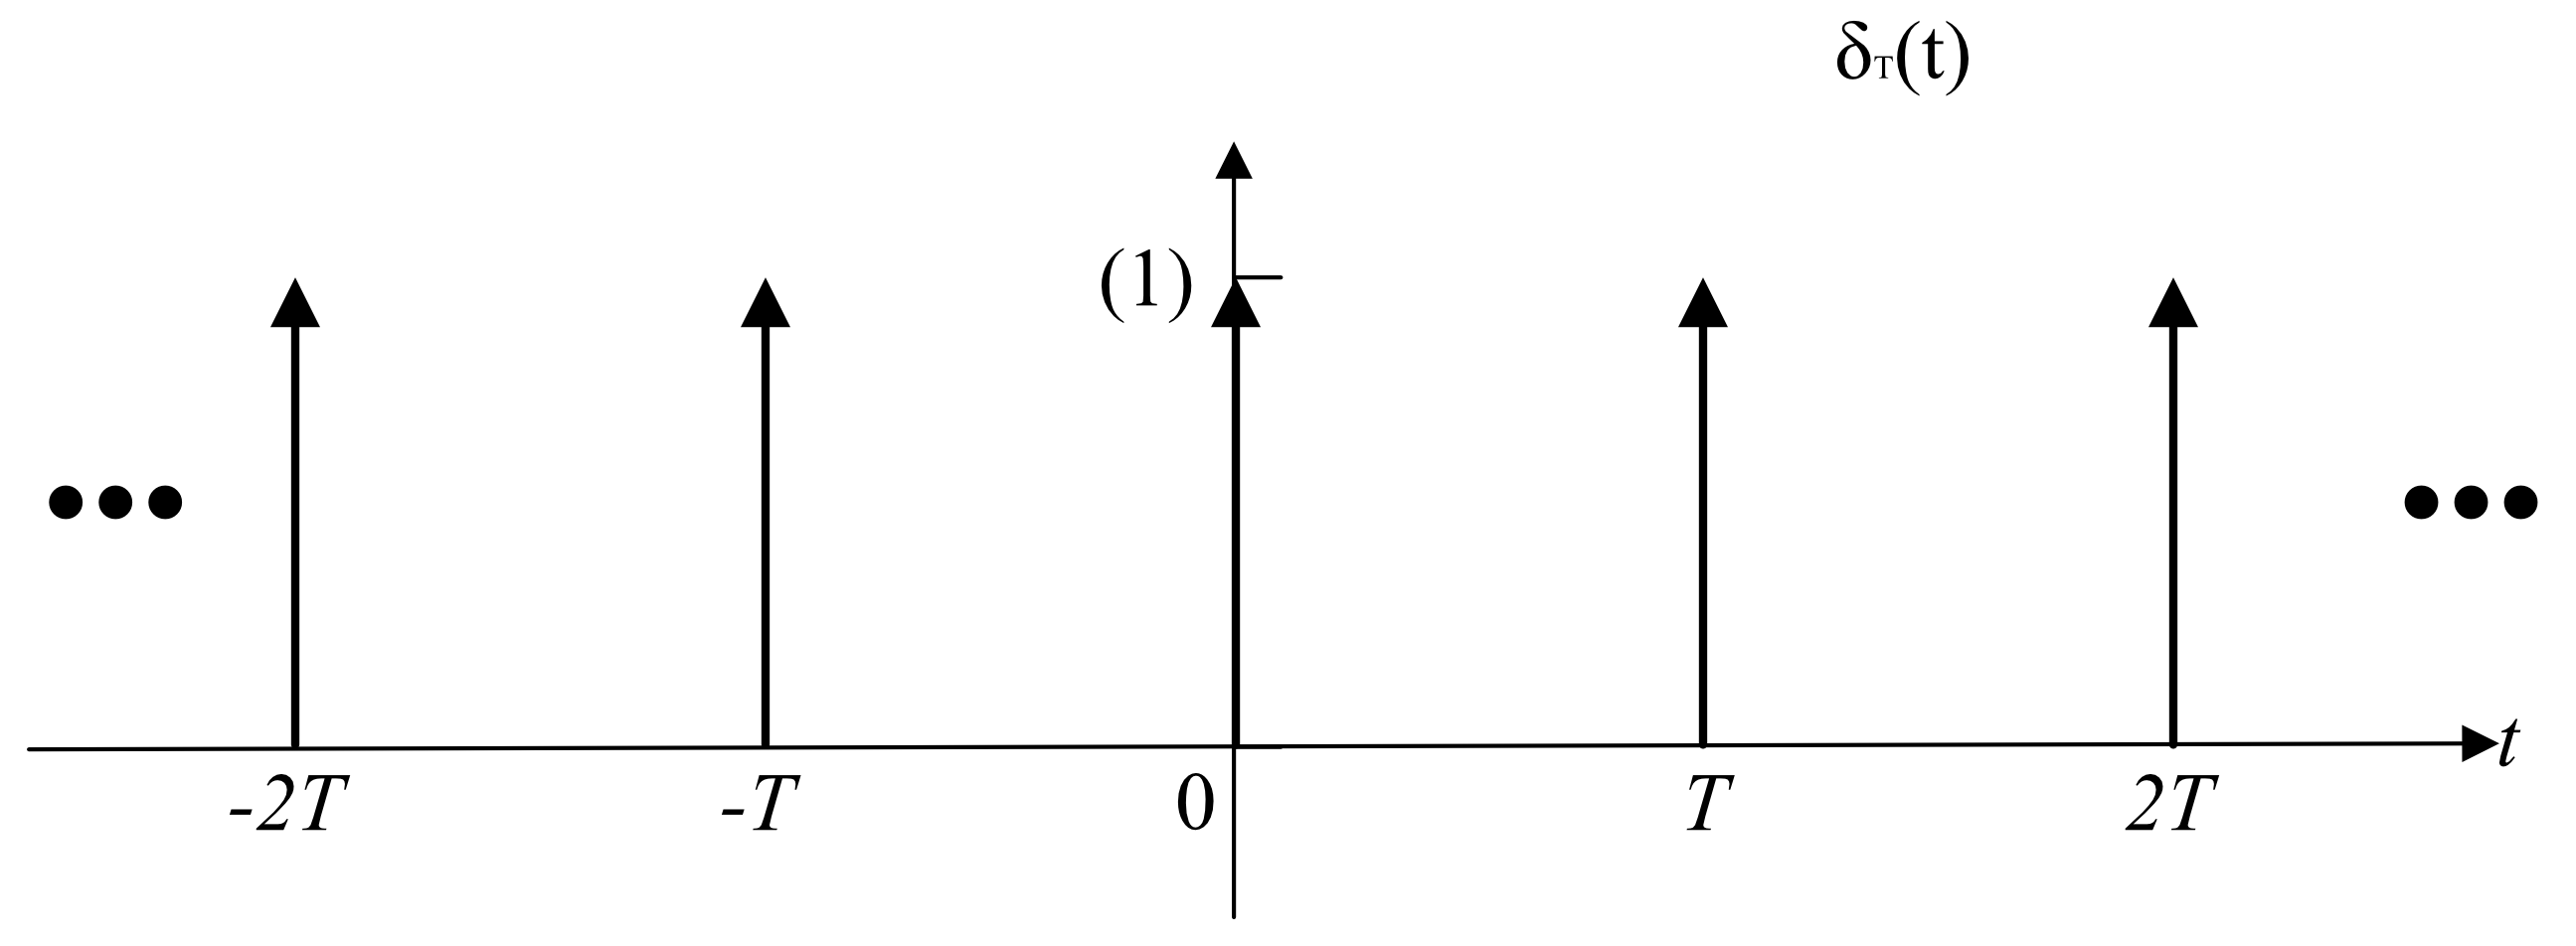
\includegraphics[width=10cm]{assets/hw4img3.png}
		\centering
	\end{figure}
\quad
\end{problem}

\end{document}